\documentclass[a4paper, 12pt, final]{article}
\usepackage{tikz}
\usepackage{fontspec}
\usepackage[margin=1.75cm]{geometry}
\usepackage{xcolor}
\usepackage{color}
\usepackage{graphicx}

\setmainfont{DejaVu Sans}
\newfontfamily{\ArialBlack}{Arial Black}
\definecolor{left}{HTML}{ffffff}
\definecolor{right}{HTML}{afbee3}

\begin{document}
\begin{tikzpicture}[remember picture, overlay]%
\node[shading = axis, rectangle, left color=left, right color=right, shading angle=110, anchor=north, minimum width=\paperwidth,
    minimum height=\paperheight] (box) at (current page.north){};%
\end{tikzpicture}%

\large\centering

\noindent{\fontsize{36pt}{36pt}\selectfont\ArialBlack STOP USING FLOATS\par}

\def\DOT{\fontsize{30pt}{30pt}\selectfont\raisebox{-6pt}{•}\kern-2pt}
\begin{itemize}
\item[\DOT] BINARY DATA WAS NOT SUPPOSED TO HAVE DECIMAL PARTS
\item[\DOT] YEARS OF COMPILER DEVELOPMENT yet NO REAL-WORLD USE FOUND for anything other than \texttt{char} and \texttt{int}
\item[\DOT] Wanted to use decimal numbers anyway for a laugh? We had a tool for that: It was called FIXED-POINT ARITHMETIC
\item[\DOT] ‘\texttt{x==x} can be FALSE’, ‘$\frac1 0$ is a number’, ‘the sum of $\frac1{10}$
and $\frac2{10}$ is\\$0.30000000004$’—statements dreamt up by the utterly Deranged
\end{itemize}

\noindent
LOOK at what Floating-Point Numbers have been demanding your Respect for all this time,
with all the circuits and data types we built for them\\
\textbf{(This is REAL Floating-Point Arithmetic, done by REAL computers)}:\medskip

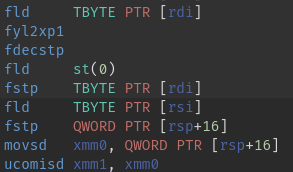
\includegraphics[height=4cm]{/home/ae/projects/float-meme/float1.png}
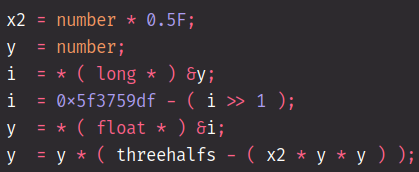
\includegraphics[height=4cm]{/home/ae/projects/float-meme/float3}\smallskip

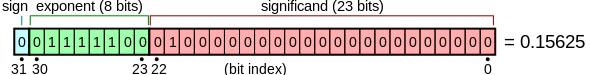
\includegraphics[height=2cm]{/home/ae/projects/float-meme/float4.png}\bigskip

\noindent ‘Hello, I want to know if \texttt{f} is a real number and less than \texttt{-1} please?’\\
‘Sure, that’ll be \texttt{f!=f?0:-1/0.f==f||f==-1.f/0?0:-1.f>f}’\medskip

\noindent
\textbf{They have played us for absolute fools}

\end{document}
